% Options for packages loaded elsewhere
\PassOptionsToPackage{unicode}{hyperref}
\PassOptionsToPackage{hyphens}{url}
\PassOptionsToPackage{dvipsnames,svgnames,x11names}{xcolor}
%
\documentclass[
  letterpaper,
  DIV=11,
  numbers=noendperiod]{scrartcl}

\usepackage{amsmath,amssymb}
\usepackage{iftex}
\ifPDFTeX
  \usepackage[T1]{fontenc}
  \usepackage[utf8]{inputenc}
  \usepackage{textcomp} % provide euro and other symbols
\else % if luatex or xetex
  \usepackage{unicode-math}
  \defaultfontfeatures{Scale=MatchLowercase}
  \defaultfontfeatures[\rmfamily]{Ligatures=TeX,Scale=1}
\fi
\usepackage{lmodern}
\ifPDFTeX\else  
    % xetex/luatex font selection
\fi
% Use upquote if available, for straight quotes in verbatim environments
\IfFileExists{upquote.sty}{\usepackage{upquote}}{}
\IfFileExists{microtype.sty}{% use microtype if available
  \usepackage[]{microtype}
  \UseMicrotypeSet[protrusion]{basicmath} % disable protrusion for tt fonts
}{}
\makeatletter
\@ifundefined{KOMAClassName}{% if non-KOMA class
  \IfFileExists{parskip.sty}{%
    \usepackage{parskip}
  }{% else
    \setlength{\parindent}{0pt}
    \setlength{\parskip}{6pt plus 2pt minus 1pt}}
}{% if KOMA class
  \KOMAoptions{parskip=half}}
\makeatother
\usepackage{xcolor}
\setlength{\emergencystretch}{3em} % prevent overfull lines
\setcounter{secnumdepth}{5}
% Make \paragraph and \subparagraph free-standing
\makeatletter
\ifx\paragraph\undefined\else
  \let\oldparagraph\paragraph
  \renewcommand{\paragraph}{
    \@ifstar
      \xxxParagraphStar
      \xxxParagraphNoStar
  }
  \newcommand{\xxxParagraphStar}[1]{\oldparagraph*{#1}\mbox{}}
  \newcommand{\xxxParagraphNoStar}[1]{\oldparagraph{#1}\mbox{}}
\fi
\ifx\subparagraph\undefined\else
  \let\oldsubparagraph\subparagraph
  \renewcommand{\subparagraph}{
    \@ifstar
      \xxxSubParagraphStar
      \xxxSubParagraphNoStar
  }
  \newcommand{\xxxSubParagraphStar}[1]{\oldsubparagraph*{#1}\mbox{}}
  \newcommand{\xxxSubParagraphNoStar}[1]{\oldsubparagraph{#1}\mbox{}}
\fi
\makeatother

\usepackage{color}
\usepackage{fancyvrb}
\newcommand{\VerbBar}{|}
\newcommand{\VERB}{\Verb[commandchars=\\\{\}]}
\DefineVerbatimEnvironment{Highlighting}{Verbatim}{commandchars=\\\{\}}
% Add ',fontsize=\small' for more characters per line
\usepackage{framed}
\definecolor{shadecolor}{RGB}{241,243,245}
\newenvironment{Shaded}{\begin{snugshade}}{\end{snugshade}}
\newcommand{\AlertTok}[1]{\textcolor[rgb]{0.68,0.00,0.00}{#1}}
\newcommand{\AnnotationTok}[1]{\textcolor[rgb]{0.37,0.37,0.37}{#1}}
\newcommand{\AttributeTok}[1]{\textcolor[rgb]{0.40,0.45,0.13}{#1}}
\newcommand{\BaseNTok}[1]{\textcolor[rgb]{0.68,0.00,0.00}{#1}}
\newcommand{\BuiltInTok}[1]{\textcolor[rgb]{0.00,0.23,0.31}{#1}}
\newcommand{\CharTok}[1]{\textcolor[rgb]{0.13,0.47,0.30}{#1}}
\newcommand{\CommentTok}[1]{\textcolor[rgb]{0.37,0.37,0.37}{#1}}
\newcommand{\CommentVarTok}[1]{\textcolor[rgb]{0.37,0.37,0.37}{\textit{#1}}}
\newcommand{\ConstantTok}[1]{\textcolor[rgb]{0.56,0.35,0.01}{#1}}
\newcommand{\ControlFlowTok}[1]{\textcolor[rgb]{0.00,0.23,0.31}{\textbf{#1}}}
\newcommand{\DataTypeTok}[1]{\textcolor[rgb]{0.68,0.00,0.00}{#1}}
\newcommand{\DecValTok}[1]{\textcolor[rgb]{0.68,0.00,0.00}{#1}}
\newcommand{\DocumentationTok}[1]{\textcolor[rgb]{0.37,0.37,0.37}{\textit{#1}}}
\newcommand{\ErrorTok}[1]{\textcolor[rgb]{0.68,0.00,0.00}{#1}}
\newcommand{\ExtensionTok}[1]{\textcolor[rgb]{0.00,0.23,0.31}{#1}}
\newcommand{\FloatTok}[1]{\textcolor[rgb]{0.68,0.00,0.00}{#1}}
\newcommand{\FunctionTok}[1]{\textcolor[rgb]{0.28,0.35,0.67}{#1}}
\newcommand{\ImportTok}[1]{\textcolor[rgb]{0.00,0.46,0.62}{#1}}
\newcommand{\InformationTok}[1]{\textcolor[rgb]{0.37,0.37,0.37}{#1}}
\newcommand{\KeywordTok}[1]{\textcolor[rgb]{0.00,0.23,0.31}{\textbf{#1}}}
\newcommand{\NormalTok}[1]{\textcolor[rgb]{0.00,0.23,0.31}{#1}}
\newcommand{\OperatorTok}[1]{\textcolor[rgb]{0.37,0.37,0.37}{#1}}
\newcommand{\OtherTok}[1]{\textcolor[rgb]{0.00,0.23,0.31}{#1}}
\newcommand{\PreprocessorTok}[1]{\textcolor[rgb]{0.68,0.00,0.00}{#1}}
\newcommand{\RegionMarkerTok}[1]{\textcolor[rgb]{0.00,0.23,0.31}{#1}}
\newcommand{\SpecialCharTok}[1]{\textcolor[rgb]{0.37,0.37,0.37}{#1}}
\newcommand{\SpecialStringTok}[1]{\textcolor[rgb]{0.13,0.47,0.30}{#1}}
\newcommand{\StringTok}[1]{\textcolor[rgb]{0.13,0.47,0.30}{#1}}
\newcommand{\VariableTok}[1]{\textcolor[rgb]{0.07,0.07,0.07}{#1}}
\newcommand{\VerbatimStringTok}[1]{\textcolor[rgb]{0.13,0.47,0.30}{#1}}
\newcommand{\WarningTok}[1]{\textcolor[rgb]{0.37,0.37,0.37}{\textit{#1}}}

\providecommand{\tightlist}{%
  \setlength{\itemsep}{0pt}\setlength{\parskip}{0pt}}\usepackage{longtable,booktabs,array}
\usepackage{calc} % for calculating minipage widths
% Correct order of tables after \paragraph or \subparagraph
\usepackage{etoolbox}
\makeatletter
\patchcmd\longtable{\par}{\if@noskipsec\mbox{}\fi\par}{}{}
\makeatother
% Allow footnotes in longtable head/foot
\IfFileExists{footnotehyper.sty}{\usepackage{footnotehyper}}{\usepackage{footnote}}
\makesavenoteenv{longtable}
\usepackage{graphicx}
\makeatletter
\def\maxwidth{\ifdim\Gin@nat@width>\linewidth\linewidth\else\Gin@nat@width\fi}
\def\maxheight{\ifdim\Gin@nat@height>\textheight\textheight\else\Gin@nat@height\fi}
\makeatother
% Scale images if necessary, so that they will not overflow the page
% margins by default, and it is still possible to overwrite the defaults
% using explicit options in \includegraphics[width, height, ...]{}
\setkeys{Gin}{width=\maxwidth,height=\maxheight,keepaspectratio}
% Set default figure placement to htbp
\makeatletter
\def\fps@figure{htbp}
\makeatother

\KOMAoption{captions}{tableheading}
\makeatletter
\@ifpackageloaded{caption}{}{\usepackage{caption}}
\AtBeginDocument{%
\ifdefined\contentsname
  \renewcommand*\contentsname{Table of contents}
\else
  \newcommand\contentsname{Table of contents}
\fi
\ifdefined\listfigurename
  \renewcommand*\listfigurename{List of Figures}
\else
  \newcommand\listfigurename{List of Figures}
\fi
\ifdefined\listtablename
  \renewcommand*\listtablename{List of Tables}
\else
  \newcommand\listtablename{List of Tables}
\fi
\ifdefined\figurename
  \renewcommand*\figurename{Figure}
\else
  \newcommand\figurename{Figure}
\fi
\ifdefined\tablename
  \renewcommand*\tablename{Table}
\else
  \newcommand\tablename{Table}
\fi
}
\@ifpackageloaded{float}{}{\usepackage{float}}
\floatstyle{ruled}
\@ifundefined{c@chapter}{\newfloat{codelisting}{h}{lop}}{\newfloat{codelisting}{h}{lop}[chapter]}
\floatname{codelisting}{Listing}
\newcommand*\listoflistings{\listof{codelisting}{List of Listings}}
\makeatother
\makeatletter
\makeatother
\makeatletter
\@ifpackageloaded{caption}{}{\usepackage{caption}}
\@ifpackageloaded{subcaption}{}{\usepackage{subcaption}}
\makeatother

\ifLuaTeX
  \usepackage{selnolig}  % disable illegal ligatures
\fi
\usepackage{bookmark}

\IfFileExists{xurl.sty}{\usepackage{xurl}}{} % add URL line breaks if available
\urlstyle{same} % disable monospaced font for URLs
\hypersetup{
  pdftitle={Weather Comparison Across Australian Cities},
  pdfauthor={Siddhi Jadhav; Sanch Anand; Thi Lan Anh Tran},
  colorlinks=true,
  linkcolor={blue},
  filecolor={Maroon},
  citecolor={Blue},
  urlcolor={Blue},
  pdfcreator={LaTeX via pandoc}}


\title{Weather Comparison Across Australian Cities}
\author{Siddhi Jadhav \and Sanch Anand \and Thi Lan Anh Tran}
\date{2025-05-27}

\begin{document}
\maketitle

\renewcommand*\contentsname{Table of Contents}
{
\hypersetup{linkcolor=}
\setcounter{tocdepth}{2}
\tableofcontents
}

\newpage

\section{Executive Summary}\label{executive-summary}

This report analyzes weather patterns across major Australian cities
using the
\href{https://www.kaggle.com/datasets/jsphyg/weather-dataset-rattle-package/data}{Rattle
weather dataset}. Key variables such as temperature, rainfall, and
humidity were compared to uncover regional climate differences. The
findings reveal distinct climate characteristics aligned with
Australia's diverse geography. These insights can support climate
planning, tourism, lifestyle decisions, and future research.

\section{Introduction}\label{introduction}

Australia is known for its diverse climates, ranging from tropical in
the north to temperate in the south. This variability impacts
agriculture, urban planning, and public health.

In this report, we compare weather characteristics across ten Australian
cities using daily data from the weatherAUS dataset. The selected cities
represent different climate zones, including tropical (Darwin), arid
(Adelaide), and temperate (Melbourne, Hobart). The dataset includes over
10 years of weather observations, providing a robust basis for analysis.
Key variables of interest are temperature, rainfall, humidity, and
pressure.

These metrics reflect both short- and long-term climate trends. Through
visualization and descriptive statistics, we uncover patterns that align
with geographical locations. This work aims to support informed,
location-specific decision-making. All analysis is reproducible using R
and Quarto.

\section{Cleaning the data}\label{cleaning-the-data}

\begin{Shaded}
\begin{Highlighting}[]
\CommentTok{\# Load the dataset}
\NormalTok{data }\OtherTok{\textless{}{-}} \FunctionTok{read.csv}\NormalTok{(}\StringTok{"data/weatherAUS.csv"}\NormalTok{)}
\end{Highlighting}
\end{Shaded}

\begin{Shaded}
\begin{Highlighting}[]
\CommentTok{\# 1. Drop high{-}missing columns}
\NormalTok{data }\OtherTok{\textless{}{-}}\NormalTok{ data }\SpecialCharTok{\%\textgreater{}\%}
  \FunctionTok{select}\NormalTok{(}\SpecialCharTok{{-}}\NormalTok{Evaporation, }\SpecialCharTok{{-}}\NormalTok{Sunshine, }\SpecialCharTok{{-}}\NormalTok{Cloud9am, }\SpecialCharTok{{-}}\NormalTok{Cloud3pm)}
\end{Highlighting}
\end{Shaded}

\begin{Shaded}
\begin{Highlighting}[]
\CommentTok{\# 2. Convert \textquotesingle{}Date\textquotesingle{} to Date type}
\NormalTok{data }\OtherTok{\textless{}{-}}\NormalTok{ data }\SpecialCharTok{\%\textgreater{}\%}
  \FunctionTok{mutate}\NormalTok{(}\AttributeTok{Date =} \FunctionTok{ymd}\NormalTok{(Date))}
\end{Highlighting}
\end{Shaded}

\begin{Shaded}
\begin{Highlighting}[]
\CommentTok{\# 3. Drop rows where \textquotesingle{}RainTomorrow\textquotesingle{} is missing}
\NormalTok{data }\OtherTok{\textless{}{-}}\NormalTok{ data }\SpecialCharTok{\%\textgreater{}\%}
  \FunctionTok{filter}\NormalTok{(}\SpecialCharTok{!}\FunctionTok{is.na}\NormalTok{(RainTomorrow))}
\end{Highlighting}
\end{Shaded}

\begin{Shaded}
\begin{Highlighting}[]
\CommentTok{\# 4. Drop wind direction columns}
\NormalTok{data }\OtherTok{\textless{}{-}}\NormalTok{ data }\SpecialCharTok{\%\textgreater{}\%}
  \FunctionTok{select}\NormalTok{(}\SpecialCharTok{{-}}\NormalTok{WindGustDir, }\SpecialCharTok{{-}}\NormalTok{WindDir9am, }\SpecialCharTok{{-}}\NormalTok{WindDir3pm)}

\CommentTok{\# 5. Convert RainToday and RainTomorrow to binary 0/1}
\NormalTok{data }\OtherTok{\textless{}{-}}\NormalTok{ data }\SpecialCharTok{\%\textgreater{}\%}
  \FunctionTok{mutate}\NormalTok{(}
    \AttributeTok{RainToday =} \FunctionTok{if\_else}\NormalTok{(RainToday }\SpecialCharTok{==} \StringTok{"Yes"}\NormalTok{, }\DecValTok{1}\NormalTok{, }\DecValTok{0}\NormalTok{),}
    \AttributeTok{RainTomorrow =} \FunctionTok{if\_else}\NormalTok{(RainTomorrow }\SpecialCharTok{==} \StringTok{"Yes"}\NormalTok{, }\DecValTok{1}\NormalTok{, }\DecValTok{0}\NormalTok{)}
\NormalTok{  )}

\CommentTok{\# 6. Drop any remaining NAs}
\NormalTok{data }\OtherTok{\textless{}{-}}\NormalTok{ data }\SpecialCharTok{\%\textgreater{}\%} \FunctionTok{drop\_na}\NormalTok{()}
\end{Highlighting}
\end{Shaded}

\begin{Shaded}
\begin{Highlighting}[]
\CommentTok{\# 7. Save cleaned data}
\FunctionTok{write\_csv}\NormalTok{(data, }\StringTok{"data/data\_cleaned.csv"}\NormalTok{)}
\end{Highlighting}
\end{Shaded}

\section{Methodology}\label{methodology}

The dataset used for this analysis, weatherAUS.csv, contains over
120,000 daily weather observations recorded across various Australian
cities. To ensure data quality, we removed columns with extensive
missing values, such as Evaporation and Sunshine, and dropped any
remaining rows with missing values to preserve analysis integrity. Wind
direction columns were excluded due to their limited relevance to the
city-level comparative focus. The resulting cleaned dataset, consisting
of 16 variables, enabled meaningful comparisons of weather
characteristics across regions.

The analysis focused on four primary variables: \emph{Rainfall,
Temperature at 3pm, Humidity at 3pm, and Pressure at 9am}. These were
chosen to represent precipitation, thermal patterns, atmospheric
moisture, and pressure systems respectively. The data was grouped by
Location, enabling city-wise summary statistics and comparisons. To
ensure consistency and reduce noise, we focused on cities with the
highest number of observations.

To visualize precipitation differences across cities, we generated a bar
plot of the ten cities with the highest average daily rainfall
(Figure~\ref{fig-rainfall-bar}). This figure highlights distinct
tropical patterns, especially in Darwin and Cairns. To complement this,
a detailed summary of weather metrics including temperature, humidity,
and pressure for these top 10 wettest cities is presented in Table
Table~\ref{tbl-summary-top10}

All analysis was conducted using the tidyverse and ggplot2 packages in
R, structured within a reproducible Quarto project. GitHub was used to
manage version control and collaboration, with each contributor working
in individual branches.

\begin{Shaded}
\begin{Highlighting}[]
\NormalTok{top\_rainfall }\OtherTok{\textless{}{-}}\NormalTok{ data }\SpecialCharTok{\%\textgreater{}\%}
  \FunctionTok{group\_by}\NormalTok{(Location) }\SpecialCharTok{\%\textgreater{}\%}
  \FunctionTok{summarise}\NormalTok{(}\AttributeTok{avg\_rain =} \FunctionTok{mean}\NormalTok{(Rainfall, }\AttributeTok{na.rm =} \ConstantTok{TRUE}\NormalTok{)) }\SpecialCharTok{\%\textgreater{}\%}
  \FunctionTok{arrange}\NormalTok{(}\FunctionTok{desc}\NormalTok{(avg\_rain)) }\SpecialCharTok{\%\textgreater{}\%}
  \FunctionTok{slice\_head}\NormalTok{(}\AttributeTok{n =} \DecValTok{10}\NormalTok{)}

\FunctionTok{ggplot}\NormalTok{(top\_rainfall, }\FunctionTok{aes}\NormalTok{(}\AttributeTok{x =} \FunctionTok{reorder}\NormalTok{(Location, avg\_rain), }\AttributeTok{y =}\NormalTok{ avg\_rain)) }\SpecialCharTok{+}
  \FunctionTok{geom\_col}\NormalTok{(}\AttributeTok{fill =} \StringTok{"burlywood3"}\NormalTok{) }\SpecialCharTok{+}
  \FunctionTok{coord\_flip}\NormalTok{() }\SpecialCharTok{+}
  \FunctionTok{labs}\NormalTok{(}\AttributeTok{x =} \StringTok{"City"}\NormalTok{, }\AttributeTok{y =} \StringTok{"Average Rainfall (mm)"}\NormalTok{)}
\end{Highlighting}
\end{Shaded}

\begin{figure}[H]

\centering{

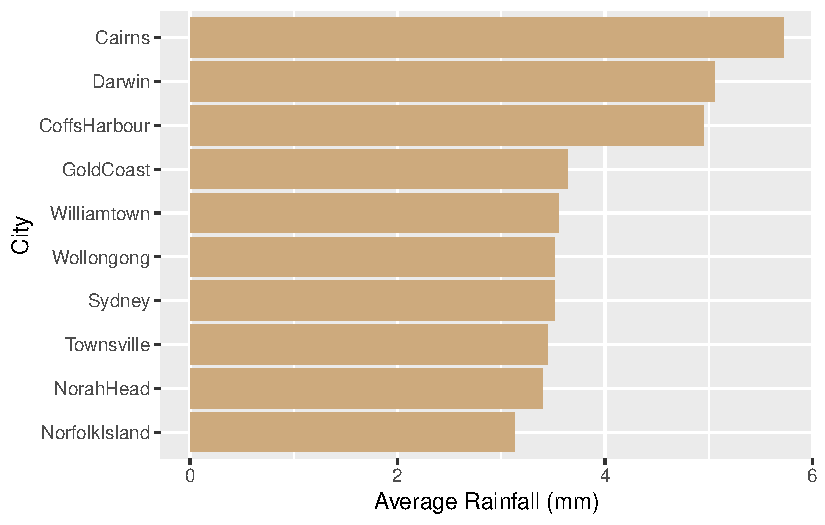
\includegraphics{report_files/figure-pdf/fig-rainfall-bar-1.pdf}

}

\caption{\label{fig-rainfall-bar}Top 10 cities by average daily rainfall
(mm)}

\end{figure}%

\begin{Shaded}
\begin{Highlighting}[]
\NormalTok{top\_cities }\OtherTok{\textless{}{-}}\NormalTok{ top\_rainfall}\SpecialCharTok{$}\NormalTok{Location}

\NormalTok{data }\SpecialCharTok{\%\textgreater{}\%}
  \FunctionTok{filter}\NormalTok{(Location }\SpecialCharTok{\%in\%}\NormalTok{ top\_cities) }\SpecialCharTok{\%\textgreater{}\%}
  \FunctionTok{group\_by}\NormalTok{(Location) }\SpecialCharTok{\%\textgreater{}\%}
  \FunctionTok{summarise}\NormalTok{(}
    \StringTok{\textasciigrave{}}\AttributeTok{Avg Rainfall}\StringTok{\textasciigrave{}} \OtherTok{=} \FunctionTok{round}\NormalTok{(}\FunctionTok{mean}\NormalTok{(Rainfall), }\DecValTok{1}\NormalTok{),}
    \StringTok{\textasciigrave{}}\AttributeTok{Avg Temp (3pm)}\StringTok{\textasciigrave{}} \OtherTok{=} \FunctionTok{round}\NormalTok{(}\FunctionTok{mean}\NormalTok{(Temp3pm), }\DecValTok{1}\NormalTok{),}
    \StringTok{\textasciigrave{}}\AttributeTok{Avg Humidity (3pm)}\StringTok{\textasciigrave{}} \OtherTok{=} \FunctionTok{round}\NormalTok{(}\FunctionTok{mean}\NormalTok{(Humidity3pm), }\DecValTok{1}\NormalTok{),}
    \StringTok{\textasciigrave{}}\AttributeTok{Avg Pressure (9am)}\StringTok{\textasciigrave{}} \OtherTok{=} \FunctionTok{round}\NormalTok{(}\FunctionTok{mean}\NormalTok{(Pressure9am), }\DecValTok{1}\NormalTok{)}
\NormalTok{  ) }\SpecialCharTok{\%\textgreater{}\%}
\NormalTok{  knitr}\SpecialCharTok{::}\FunctionTok{kable}\NormalTok{()}
\end{Highlighting}
\end{Shaded}

\begin{longtable}[]{@{}
  >{\raggedright\arraybackslash}p{(\columnwidth - 8\tabcolsep) * \real{0.1750}}
  >{\raggedleft\arraybackslash}p{(\columnwidth - 8\tabcolsep) * \real{0.1625}}
  >{\raggedleft\arraybackslash}p{(\columnwidth - 8\tabcolsep) * \real{0.1875}}
  >{\raggedleft\arraybackslash}p{(\columnwidth - 8\tabcolsep) * \real{0.2375}}
  >{\raggedleft\arraybackslash}p{(\columnwidth - 8\tabcolsep) * \real{0.2375}}@{}}

\caption{\label{tbl-summary-top10}Summary of key weather variables in
top 10 wettest cities}

\tabularnewline

\toprule\noalign{}
\begin{minipage}[b]{\linewidth}\raggedright
Location
\end{minipage} & \begin{minipage}[b]{\linewidth}\raggedleft
Avg Rainfall
\end{minipage} & \begin{minipage}[b]{\linewidth}\raggedleft
Avg Temp (3pm)
\end{minipage} & \begin{minipage}[b]{\linewidth}\raggedleft
Avg Humidity (3pm)
\end{minipage} & \begin{minipage}[b]{\linewidth}\raggedleft
Avg Pressure (9am)
\end{minipage} \\
\midrule\noalign{}
\endhead
\bottomrule\noalign{}
\endlastfoot
Cairns & 5.7 & 27.9 & 61.7 & 1014.2 \\
CoffsHarbour & 5.0 & 22.3 & 62.3 & 1018.3 \\
Darwin & 5.1 & 31.1 & 51.7 & 1011.9 \\
GoldCoast & 3.6 & 23.7 & 62.8 & 1018.0 \\
NorahHead & 3.4 & 20.8 & 67.5 & 1018.3 \\
NorfolkIsland & 3.1 & 20.4 & 67.8 & 1017.7 \\
Sydney & 3.5 & 21.8 & 54.3 & 1018.3 \\
Townsville & 3.4 & 27.8 & 57.3 & 1015.2 \\
Williamtown & 3.6 & 22.7 & 53.2 & 1018.4 \\
Wollongong & 3.5 & 19.9 & 65.1 & 1018.1 \\

\end{longtable}

\section{Results}\label{results}

Figure Figure~\ref{fig-temp-boxplot} displays the 3pm temperature
distribution by observation count for the top 10 Australian cities. The
tropical, desert, and temperate regions of Australia are clearly
distinguished by this research.

Tropical and desert climate conditions are reflected in the highest and
most stable afternoon temperatures found in cities like \textbf{Darwin}
and \textbf{Alice Springs}. Smaller interquartile ranges are seen in
these cities, suggesting hot, consistent weather that is typical of the
area. Conversely, cities with temperate, coastal climates, such as
\textbf{Hobart}, \textbf{Melbourne}, and \textbf{Sydney}, show higher
variability and cooler median temperatures. Cities like \textbf{Perth}
and \textbf{Brisbane} have outliers, indicating sporadic excessive
temperature events that may be caused by particular weather systems.

All things considered, the boxplot illustrates how Australia's varied
topography affects temperature distributions. While southern and coastal
towns exhibit milder and more diverse climates, northern cities are
often hotter and more stable. These findings show how latitude,
altitude, and proximity to the coast affect temperature trends and are
consistent with the anticipated climatic variation throughout Australia.

\begin{Shaded}
\begin{Highlighting}[]
\NormalTok{top10 }\OtherTok{\textless{}{-}}\NormalTok{ data }\SpecialCharTok{\%\textgreater{}\%}
  \FunctionTok{count}\NormalTok{(Location, }\AttributeTok{sort =} \ConstantTok{TRUE}\NormalTok{) }\SpecialCharTok{\%\textgreater{}\%}
  \FunctionTok{slice\_head}\NormalTok{(}\AttributeTok{n =} \DecValTok{10}\NormalTok{) }\SpecialCharTok{\%\textgreater{}\%}
  \FunctionTok{pull}\NormalTok{(Location)}

\NormalTok{data }\SpecialCharTok{\%\textgreater{}\%}
  \FunctionTok{filter}\NormalTok{(Location }\SpecialCharTok{\%in\%}\NormalTok{ top10) }\SpecialCharTok{\%\textgreater{}\%}
  \FunctionTok{ggplot}\NormalTok{(}\FunctionTok{aes}\NormalTok{(}\AttributeTok{x =}\NormalTok{ Location, }\AttributeTok{y =}\NormalTok{ Temp3pm)) }\SpecialCharTok{+}
  \FunctionTok{geom\_boxplot}\NormalTok{(}\AttributeTok{fill =} \StringTok{"pink"}\NormalTok{) }\SpecialCharTok{+}
  \FunctionTok{labs}\NormalTok{(}\AttributeTok{x =} \StringTok{"City"}\NormalTok{, }\AttributeTok{y =} \StringTok{"Temperature at 3pm (°C)"}\NormalTok{) }\SpecialCharTok{+}
  \FunctionTok{theme}\NormalTok{(}\AttributeTok{axis.text.x =} \FunctionTok{element\_text}\NormalTok{(}\AttributeTok{angle =} \DecValTok{45}\NormalTok{, }\AttributeTok{hjust =} \DecValTok{1}\NormalTok{))}
\end{Highlighting}
\end{Shaded}

\begin{figure}[H]

\centering{

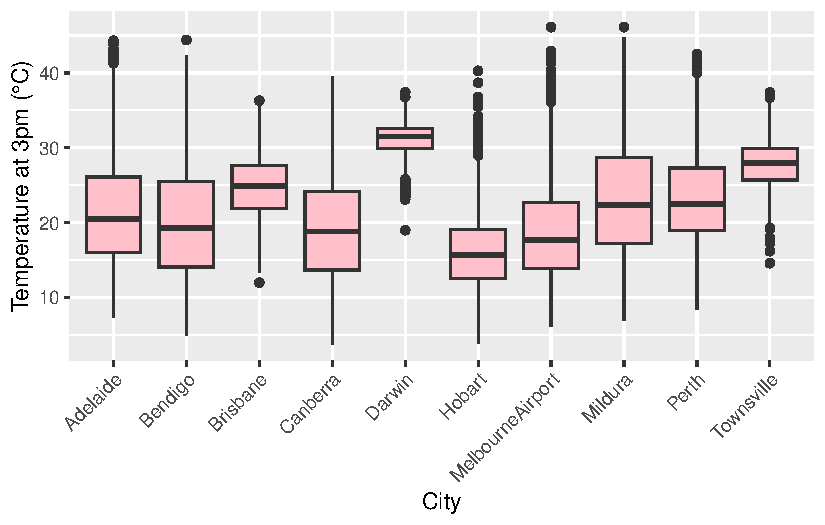
\includegraphics{report_files/figure-pdf/fig-temp-boxplot-1.pdf}

}

\caption{\label{fig-temp-boxplot}Distribution of 3pm temperatures across
the top 10 Australian cities by observation count, highlighting
differences between tropical and temperate regions.}

\end{figure}%

As shown in Figure~\ref{fig-temp-boxplot} cities such as Darwin and
Alice Springs experience the highest and most consistent afternoon
temperatures. On the other hand, Melbourne and Hobart show cooler and
more varied temperature distributions. This supports the expected
climatic variation between Australia's tropical north and temperate
south.

\section{Discussion}\label{discussion}

This analysis highlights the significant climatic diversity across
Australian cities:

\begin{itemize}
\item
  \textbf{Rainfall Patterns}: Cities in tropical and coastal regions,
  such as Cairns and Darwin, receive the highest average rainfall (see
  Figure~\ref{fig-rainfall-bar}), confirming the impact of geography on
  precipitation. The consistent presence of coastal cities in the top 10
  list indicates the influence of sea moisture and oceanic weather
  systems.
\item
  \textbf{Temperature and Humidity}: Tropical cities like Darwin and
  Cairns are not only warmer but also exhibit less variability in daily
  temperatures. This is typical for equatorial climates. In contrast,
  temperate cities such as Melbourne and Hobart experience cooler and
  more fluctuating weather, influenced by dynamic weather fronts.
\item
  \textbf{Air Pressure Observations}: Most cities show similar
  atmospheric pressure, except Darwin, where lower pressure may
  contribute to the region's tropical climate and higher rainfall.
\item
  \textbf{Temperature Distribution}: The boxplot reinforces (see
  Figure~\ref{fig-temp-boxplot}) how geography affects temperature:
  inland cities are hot and stable, while southern cities are cooler and
  more variable. Outliers and wider spreads reflect occasional weather
  extremes in cities like Melbourne and Sydney.
\end{itemize}

\section{Conclusion}\label{conclusion}

In summary, the climate of Australian cities varies significantly by
location. Northern and inland areas such as Darwin and Alice Springs are
warmer and more stable in temperature, while southern and coastal cities
like Melbourne, Hobart, and Sydney exhibit cooler, more variable
weather. High rainfall is concentrated in tropical and coastal regions,
confirming expected climate zones. These findings align with known
climate patterns across the country.

\section{Recommendations}\label{recommendations}

\begin{itemize}
\item
  \textbf{For Climate Planning}: City planners and infrastructure
  developers should consider local rainfall and temperature variability
  when designing drainage systems, buildings, and energy
  systems---especially in high-rainfall cities like Cairns and Darwin.
\item
  \textbf{For Tourism and Lifestyle Choices}: Tourists and residents
  seeking stable warm weather may prefer Darwin or Alice Springs. Those
  sensitive to temperature variability may find southern cities less
  comfortable.
\item
  \textbf{For Future Research}:

  \begin{itemize}
  \item
    \textbf{Incorporate Time Dimension}: Explore seasonal or monthly
    trends to observe how rainfall and temperature vary over time.
  \item
    \textbf{Visualise More Variables}: Add plots for humidity,
    temperature, or pressure to deepen comparison across cities.
  \item
    \textbf{Explore Extreme Events}: Analyse maximum rainfall or
    temperature to assess weather extremes and risks.
  \item
    \textbf{Forecast rain tomorrow}: Predict whether it will rain
    tomorrow based on other variables from previous records.
  \end{itemize}
\end{itemize}

\section{References}\label{references}

Wickham H, Averick M, Bryan J, Chang W, McGowan LD, François R,
Grolemund G, Hayes A, Henry L, Hester J, Kuhn M, Pedersen TL, Miller E,
Bache SM, Müller K, Ooms J, Robinson D, Seidel DP, Spinu V, Takahashi K,
Vaughan D, Wilke C, Woo K, Yutani H (2019). ``Welcome to the
tidyverse.'' \emph{Journal of Open Source Software}, \emph{4}(43), 1686.
doi:10.21105/joss.01686 \url{https://doi.org/10.21105/joss.01686}.

H. Wickham. ggplot2: Elegant Graphics for Data Analysis. Springer-Verlag
New York, 2016.

Young JS (2017). ``Weather Dataset (Rattle Package).'' Kaggle Datasets.
Retrieved from
https://www.kaggle.com/datasets/jsphyg/weather-dataset-rattle-package/data




\end{document}
